\documentclass[12pt]{article}
\setlength{\parskip}{\baselineskip}
\usepackage{float}
\usepackage{graphicx}
\title{Is the temperature of one year significantly correlated with the next year (successive years), across the years?}
\author{Hira Tanvir}

\begin{document}
	\maketitle
	
Hypothesis: The temperature of one year is significantly correlated with the next year.

\section{Methods}
In Key West, Florida, annual mean temperatures were collected throughout the 20th century. The aim of this practical was to find a correlation between one years temperature and the temperature of the subsquent year. This was achieved by calculating the correlation between t-1 pairs of years, where t is the total number of years. 

Firstly, the correlation coefficient was computed between successive years within an R script. Two sets of vectors, t years and t-1 years were created and the correlation was then calculated by using the function $cor(t-1,t)$.

Secondly, the correlation between t and random permutations of the time series was calculated. These correlations were compared with that of the first set.
\section{Results}	
\begin{figure}[H]
	\centering
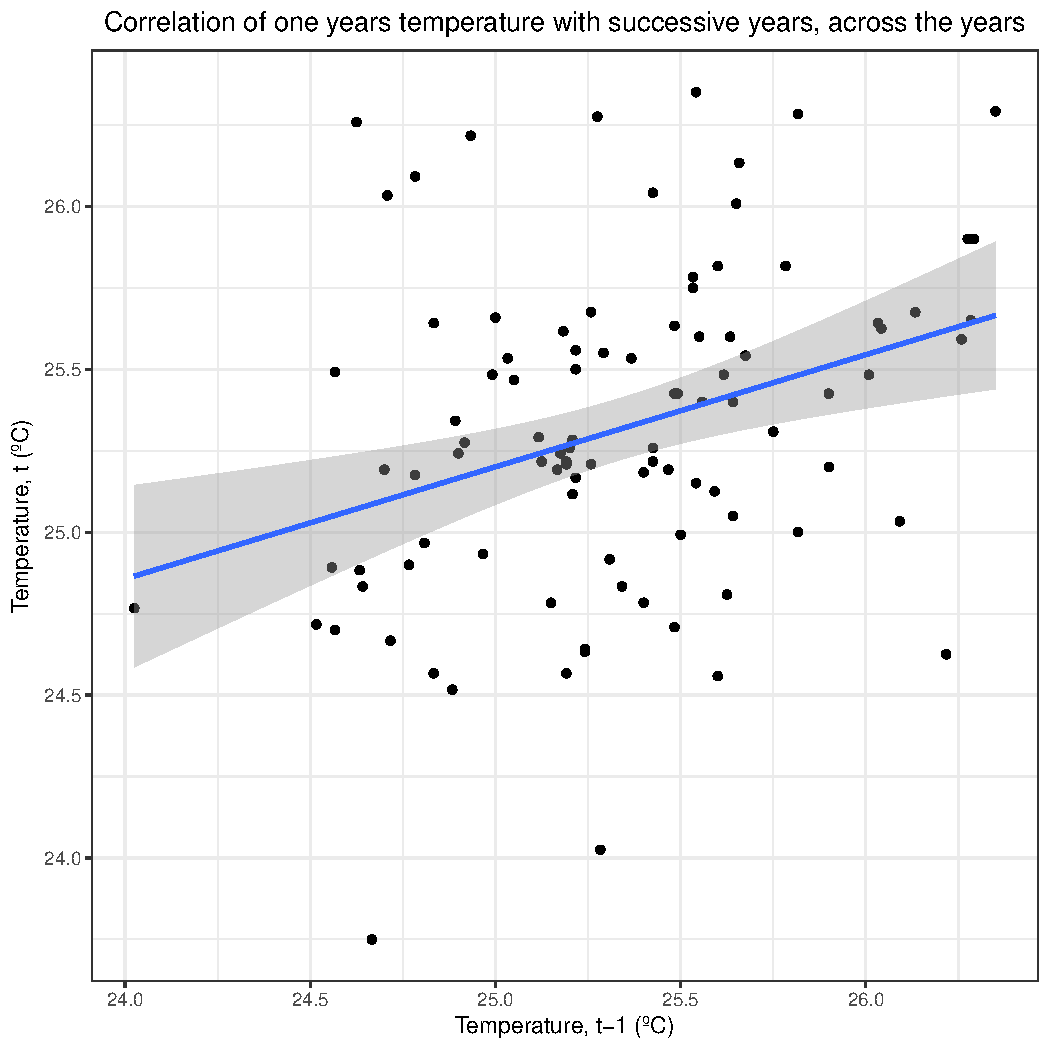
\includegraphics[scale=.5]{TAutoCorrGraph.pdf}
	\caption{Temperature in Key West, Florida for the 20th century.}
	\label{fig:TAutoCorrGraph1}
\end{figure}

\section{Interpretation}
Figure 1 shows a graph with positive correlation between t and t-1 years. The positive correlation shown in the graph is also backed up the correlation value of 0.326, which was attained by computing t and t-1 years using R's $cor() function$. We can interpret that one years temperature is positively correlated with the temperature of the following year with high significance as $p<0.005$.

\end{document}